\documentclass[10pt,a4paper]{article}
\usepackage[margin=1.8cm]{geometry}
\usepackage[T1]{fontenc}
\usepackage{lmodern,microtype,amssymb,booktabs,tabularx,xcolor,enumitem,tikz,graphicx}
\usetikzlibrary{arrows.meta,positioning}
\usepackage[hidelinks]{hyperref}
\setlist{nosep,leftmargin=*}
\setlength{\parskip}{3pt}
\setlength{\parindent}{0pt}
\setlength{\emergencystretch}{3em}
\sloppy
\newcommand{\tool}[1]{\texttt{#1}}

\title{\vspace{-1.2cm}\textbf{Graph Analytics Orchestrator}\\[2pt]\large CS6855 Course Project --- Group 2 Report}
\author{\small Pallepogu Rishi (CS23B048) \quad Abhinand Shaji (ED22B044) \quad
Pervaje Surya Prasad Bhat (ED23B035)\\ \small Syed Sufiyan (NS26Z168) \quad Mohd Hamza (PH22B016)}
\date{November 6, 2026}

\begin{document}
\maketitle
\vspace{-0.8cm}

\section{Overview}
Our LangGraph orchestrator answers natural-language questions over five provided datasets
(\tool{airports}, \tool{karate}, \tool{lesmis}, \tool{courses}, \tool{projects}). It discovers a curated
selection of Assignment~3 tools by reading their manifests rather than hard-coding query-to-tool mappings.
Google Gemini supplies structured plans through its OpenAI-compatible API; \tool{LLM\_MODEL} configures the model
and \tool{LLM\_API\_KEY} supplies the key through the environment. The required entry point is
\texttt{python run\_queries.py -{}-queries <file> -{}-out answers.json}.

\section{Design}
\begin{center}
\resizebox{\linewidth}{!}{%
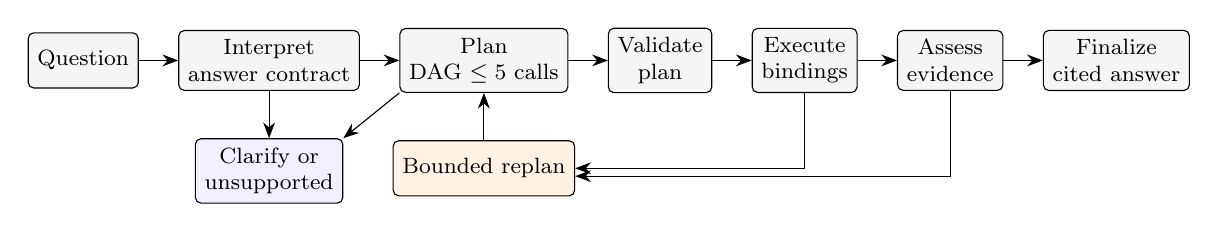
\begin{tikzpicture}[node distance=4mm and 5mm, every node/.style={font=\footnotesize},
  box/.style={draw, rounded corners=2pt, align=center, minimum height=7mm, fill=gray!8},
  arr/.style={-{Stealth[length=2mm]}}]
\node[box] (q) {Question};
\node[box, right=of q] (i) {Interpret\\answer contract};
\node[box, right=of i] (p) {Plan\\DAG $\leq 5$ calls};
\node[box, right=of p] (v) {Validate\\plan};
\node[box, right=of v] (e) {Execute\\bindings};
\node[box, right=of e] (a) {Assess\\evidence};
\node[box, right=of a] (f) {Finalize\\cited answer};
\node[box, below=6mm of p, fill=orange!10] (r) {Bounded replan};
\node[box, below=6mm of i, fill=blue!6] (c) {Clarify or\\unsupported};
\draw[arr] (q)--(i); \draw[arr] (i)--(p); \draw[arr] (p)--(v); \draw[arr] (v)--(e); \draw[arr] (e)--(a); \draw[arr] (a)--(f);
\draw[arr] (e.south) |- (r.east); \draw[arr] (a.south) |- ([yshift=-1mm]r.east); \draw[arr] (r)--(p);
\draw[arr] (i)--(c); \draw[arr] (p.south west) -- (c.north east);
\end{tikzpicture}%
}
\end{center}
\vspace{-3mm}
\begin{enumerate}
\item \textbf{Curate and discover.} Offline tests check candidate manifests, schema-valid outputs,
  repeatability, independent numerical behavior and execution time. Selected tool files are copied unchanged
  into \tool{registry/tools/}. Startup scans those manifests plus four instructor infrastructure tools; strict
  validation rejects missing or duplicate tools.
\item \textbf{Interpret.} A forced structured response produces an immutable answer contract: answer type,
  cardinality, ordering, required evidence and any genuine missing user choices. A dynamic graph catalogue
  supplies exact IDs and attributes. Bounded, question-relevant label hints help identify entities such as
  the instructor and administrator, but cannot themselves support a final answer.
\item \textbf{Plan and validate.} The planner receives the contract and the discovered tool catalogue. It
  creates an acyclic plan of at most five steps or returns a structured clarification/unsupported decision.
  Validator checks include tool-name membership, manifest arguments, dependencies and graph IDs.
\item \textbf{Execute and chain.} Ready steps run on one GraphStore. JSON Pointer bindings pass a prior
  \tool{/result\_graph\_id} or resolved node ID into the next call. q19, for example, chains a Girvan--Newman
  split to PageRank on the larger registered subgraph. Tool outputs are validated before becoming evidence.
\item \textbf{Assess, finalize and recover.} Evidence assessment tests whether each contract requirement
  is supported and may request bounded replanning. The finalizer must return the required structured type
  and cite existing step IDs and output paths. JSONL traces record every LLM/tool call and final answer;
  retries, response caching, SQLite checkpoints and deterministic tool replay support interrupted batches.
\end{enumerate}

\section{Registry selection}
The local curation report evaluated \textbf{186 candidates}; 167 passed its checks and one implementation was
selected for each of \textbf{33 analytical tools}. Four infrastructure tools remain separate. Among eligible
candidates the lowest median runtime wins, with implementation ID as the tie-breaker. Selection is
machine-dependent, so the curated registry must accompany the submission. Rejected candidates were
investigated individually: some initial rejections were evaluator/output-shape false positives, not tool bugs.

\clearpage
\section{Public-set evaluation}
The public set contains 30 questions. We compare status, structured type and value against the supplied
public expectations (0.1\% tolerance for numbers; ranking order where relevant). The figures below are the
\emph{best trace-backed terminal results across recorded attempts}, not one uninterrupted run. In
particular, the old q26 clarification from \tool{answers\_public\_v5.json} was deliberately \emph{not}
selected; its later error is counted.

\begin{center}
\begin{tabularx}{0.93\linewidth}{@{}l r X@{}}
\toprule
Expected class & Correct & Selected outcomes \\
\midrule
Answerable, q01--q23 & 20/23 & 20 correct answers; q17 and q22 errored, q21 answered incorrectly. \\
Ambiguous, q24--q26 & 2/3 & q24 and q25 clarified; q26 ended in error. \\
Unsupported, q27--q30 & 4/4 & All four correctly returned unsupported. \\
\midrule
\textbf{Total} & \textbf{26/30 (86.7\%)} & 21 answered (20 correct), 2 clarification, 4 unsupported, 3 error. \\
\bottomrule
\end{tabularx}
\end{center}

The q12 answer and trace agree on a Jaccard similarity of 0.432432, so q12 is counted.
The q21 answer and trace both give c63, but that value comes from betweenness on the entire
\tool{lesmis} graph, not Valjean's circle; the expected local answer is c40. We make no
hidden-set accuracy claim. Most successful answers use one or two tools within the five-call budget.

\section{Analysis of remaining failures}
\begin{enumerate}
\item \textbf{q17: derived-subgraph scope was misjudged.} An ego-network call registered the instructor's
  local graph; degree centrality on it ranked m1 first and m2 highest among m1's friends. Evidence
  assessment mistakenly treated the result as a ranking on the whole original graph. Further replanning
  hit the limit. The assessor must honor the executed \tool{graph\_id} and exclude the instructor when
  selecting a friend.
\item \textbf{q22: wrong analysis chain.} Javert's immediate circle requires node resolution,
  \tool{ego\_network}, and \tool{motif\_count} on the resulting graph. Initial plans embedded arguments
  inside tool names; later attempts chose clustering tools and exhausted replanning. The expected count
  for the full ego subgraph is 96 triangles; a local coefficient or triangles through Javert alone
  cannot substitute for that result.
\item \textbf{q21: wrong graph for the calculation.} Betweenness was calculated on all 77
  \tool{lesmis} characters, making Myriel (c63) rank second globally. The workflow then built
  Valjean's neighbour graph without recalculating betweenness there. Instead it should calculate
  betweenness on Valjean's 37-node ego graph (including Valjean), then exclude Valjean only when
  choosing the answer. That calculation ranks Javert (c40) next, at 0.062634.
\item \textbf{q26: ambiguity incorrectly pursued as a computation.} ``How close'' could mean hops,
  co-appearance strength or neighbourhood similarity. The later run tried weighted shortest-path
  steps and ended in error rather than requesting clarification. A shared-chapter weight represents
  strength, not a distance; interpreting it as path length changes the meaning of the question.
\end{enumerate}

\clearpage
\section{Registry implementation findings}
The following were found in \emph{unselected} candidates. We did not edit registry source.
\begin{enumerate}
\item \textbf{Major correctness bug: \tool{motif\_count.7cc0c2d7}.} It returns \textbf{52}
  triangles on \tool{karate}; independent NetworkX counting and the selected implementation return
  \textbf{45}. A three-node induced subgraph gives a minimal reproducer:
\begin{verbatim}
sub = store.subgraph("karate", ["m2", "m3", "m14"], "repro")   # one triangle
tool.run(store, graph_id=sub)["result"]["triangle_count"]  # 2, expected 1
\end{verbatim}
  The implementation orders two nodes by their positions in \tool{g.nodes()} but filters the third
  using a string comparison of node IDs. These orderings differ for IDs such as \tool{m14} and
  \tool{m2}, causing double counting. It should use one consistent node order. No modification was
  made to the student tool.
\item \textbf{Smaller contract bug: \tool{minimum\_spanning\_tree.5c98c8eb}.} A valid
  \tool{lesmis}, \tool{top\_k=100} call serializes to \textbf{8,717 bytes}, above the required
  \textbf{8,192-byte} output ceiling. Its result selection limits item count, not serialized size.
\item \textbf{Minor limitation, not a wrong result: \tool{maximal\_cliques.ab9fb3a3}.}
  A valid \tool{top\_k=100} Karate request returns an explicit size-limit error rather than a
  bounded preview. It does not return an incorrect clique or violate the output-size limit.
\end{enumerate}
Other candidates rejected by the initial harness were tested against their actual result shapes;
false-positive rejections are not presented as bugs. Verified issues can be reported through the
course's discussion channel without sharing source code.

\section{Member contributions}
\begin{itemize}
\item \textbf{Abhinand Shaji (ED22B044):} Improved executor reliability during replanning by reusing a unique node ID from prior evidence when the tool and graph match, and constrained generated node arguments to exact entity hints or dependency outputs. Added regression coverage for this behavior. Investigated q26's ambiguity, clarified that ``close'' requires a chosen metric (fewest hops, weighted distance, or similarity), and added tests for clarification and unweighted shortest paths.
\item \textbf{Syed Sufiyan (NS26Z168):} Orchestrator integration and public-set evaluation;
  Assignment~3 node-similarity, diameter/eccentricity and betweenness implementations.
\item \textbf{Mohd Hamza (PH22B016):} Code review and independent reference checks, failure analysis,
  registry bug investigation and clean-setup review. Wrote this report.
\end{itemize}

\textbf{AI-use acknowledgment.} AI-assisted coding was used. The group remains responsible for
validating its outputs and explaining the submitted implementation.
\end{document}
